\documentclass[12pt]{article}
\usepackage{tikz}
\usepackage{amsmath}
\usepackage{float}
\usepackage{array}
\usepackage{cancel}

\title{Powers and Roots Course\\
\begin{center}

\includegraphics[width=4em]{ApS_logo.png}
\end{center}
\begin{normalsize}Tutoring Centre Ferndale \end{normalsize}}
\author{}
\date{}

\begin{document}
\maketitle

\section*{Powers and Roots}

\paragraph{Power}
Power means size and strength.\\

\begin{enumerate}

\item What does power mean, in your own words?
\item use power in a sentence.

\paragraph{Powers of Numbers}
When a number is multiplied by itself over and over, you raise it to a higher power. It gets bigger and it is called a power of that number.

\vspace{14pt}
An example is the powers of 3:

The first power of 3 is just 3.

The second power of 3 is $3 \times 3 = 9.$

The third power of 3 is $3 \times 3 \times 3 = 27.$

\vspace{14pt}
And so on. You get the idea?

\item What does the powers of a number mean, in your own words?
\item Write 3 examples of the powers of a number..

\paragraph{Root}
Root means the base of something or where things grow from, like the root of a tree.

\item What does root mean, in your own words?
\item Use root in a sentence that shows its meaning.

\paragraph{Roots of Numbers}
The number being multiplied is called the root, and the number of times it is multiplied by itself is called the power.\\

\begin{center}
$3 \times 3 \times 3$\\
$3 \times 3$\\
$3$
\end{center}

\item What is meant by the root of a number, in your own words?
\item Write 3 examples of the root of a number.

\subsection*{Writing Powers}

You write the power as a small raised number to the right of the root.

\begin{center}
$\text{root}\rightarrow$
{\fontsize{30}{34}\selectfont 3}
$\textsuperscript{{\fontsize{15}{20}\selectfont 5} \ \raisebox{1.5ex}{$\longleftarrow$\ }}\raisebox{0.8ex}{\textsuperscript{\normalsize{\text{power}}}}$
\normalsize
\end{center}

It's written that way because it's shorter, rather than having to write out in full that number of multiplications, so $3^5 \text{ means }3 \times 3 \times 3 \times 3 \times 3.$\\

\item Write 5 examples of a power of a number being written this way
\item Label them with arrows pointing to the root and to the power.

\subsection*{Reading Powers}

When you are reading a number that is written with a power, such as $3^5$, there are a few different ways of saying it.\\

You can call it the fifth power of 3.\\

You can say 3 to the power of 5.\\

You can say 3 raised to the fifth power.\\

You can say 3 to the fifth power.\\

Or you can just say 3 to the fifth.

\item Read these powers out loud: $3^5, 2^2, 6^4, 8^5, 7^8.$

\subsection*{Index}
Index means a pointer, like the index of a book points to where you can find things in it.

\item What is an index, in your own words?
\item Use index in a sentence.

\paragraph{Index of a Number}
The power of a number can also be called the index because it points to what power the number is being raised to.\\

For example, the powers of 3 are $3^1=3, 3^2=9, 3^3=27, 3^4=81$ and $3^5=273$ so you could say that the $4^{th}$ power of 3 is 81, with 4 being the pointer to that particular power.\\

\begin{center}
$\text{root}\rightarrow$
{\fontsize{30}{34}\selectfont 3}
$\textsuperscript{{\fontsize{15}{20}\selectfont 5} \ \raisebox{1.5ex}{$\longleftarrow$\ }}\raisebox{0.8ex}{\textsuperscript{\normalsize{\text{index}}}}$
\normalsize
\end{center}

\item What is the index of a number, in your own words?
\item Use index in a sentence that show this meaning.

\paragraph{Indices}
If you are talking about more than one index you don’t say indexes. The 2 and the 3 in $5^2+6^3$ are called indices, and you say it as \textit{indisees.} Index is  a Latin word so it follows the Latin language's rules for making plurals.

\item What are indices, in your own words?
\item Use indices in  a sentence.

\paragraph{Exponent}
Exponent means a person or thing which explains or makes clear.\\

It is from Latin ex, meaning out of, and ponere, meaning place, with the idea of laying something out to view it's parts.\\

 For example, "The speaker is an exponent of the need for clean energy."\\
 
\item What does exponent mean, in your own words?
\item Use exponent in a sentence.

\paragraph{Exponent of a Number}
In maths, most of the world calls it the index or the power, but exponent is the preferred word in the US.\\

\begin{center}
$\text{root}\rightarrow$
{\fontsize{30}{34}\selectfont 3}
$\textsuperscript{{\fontsize{15}{20}\selectfont 5} \ \raisebox{1.5ex}{$\longleftarrow$\ }}\raisebox{0.8ex}{\textsuperscript{\normalsize{\text{exponent}}}}$
\normalsize
\end{center}

\item What is the exponent of a number, in your own words?
\item Use exponent in a sentence, showing this meaning.

\paragraph{The {\fontsize{30}{34}\selectfont {\raisebox{-.8ex}{\textasciicircum}}} Caret}
Sometimes when writing indices on a computer, because we are using a keyboard which only allows the use of certain characters, instead of the small raised number we use the {\fontsize{30}{34}\selectfont {\raisebox{-.8ex}{\textasciicircum}}} \ 'caret' symbol. $3^5$ would be written as 3{\fontsize{30}{34}\selectfont {\raisebox{-.8ex}{\textasciicircum}}}5. The caret symbol is also called a circumflex or a hat.\\

\item Write 5 examples of a power of a number using a caret.
\item Label your examples with arrows pointing to the root and to the power.
\item When might you have to write a power of a number with a caret?


\subsection*{Squares}

A square has sides of equal length.\\

\item What is a square, in your own words?
\item Use square in a sentence.

\paragraph{Area}
Area means the size of a flat surface.\\

\item What is area, in your own words?
\item Use area in a sentence.

To find the area of a square you multiply the length of the two sides.\\

\item What is the area of a square that has sides of 5 cm?

\begin{figure}
  \centering
  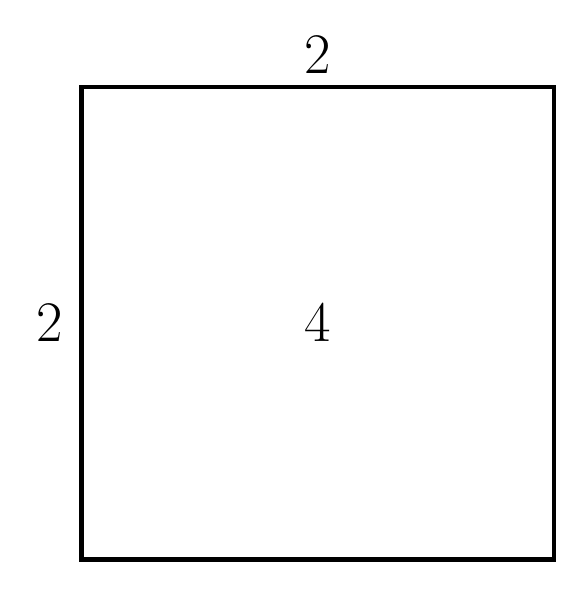
\begin{tikzpicture}
    \draw [ultra thick](0,0) rectangle (6,6);
%    \fill[lightgray] (0,0) rectangle (6,6);
    \node at (3,3) {\fontsize{20}{24}\selectfont 4};
    \node at (-0.4,3) {\fontsize{20}{24}\selectfont 2};
    \node at (3,6.4) {\fontsize{20}{24}\selectfont 2};
  \end{tikzpicture}
  \quad
  \begin{minipage}{5cm}
    \[
    \text{Area} = 2 \times 2 = 2^2 = 4
    \]
  \end{minipage}
\end{figure}

That's why multiplying a number by itself is called squaring the number.\\

You wouldn't call it 2 to the second power or anything. You would say the square of 2 is 4 or that 2 squared is 4.

\item How do you read "$6^2$"?

\subsection*{Cubes}

\paragraph{Volume}
Volume means the size of something and how much space it takes up, not just a flat area.\\

\item What does volume mean, in your own words?
\item Use volume in a sentence.

A cube has 3 sides all of the same length.

\item What is a cube, in your own words?
\item Use cube in a sentence.

To find the volume of a cube, how big it is, you multiply the length of its side by itself 3 times.\\

\item What is the volume of a cube that has 5cm sides?

That's why a number that has been multiplied by itself 3 times is called the cube of that number. Rather than saying "2 to the power of 3 is 8," you would say the cube of 2 is 8, or 2 cubed is 8.

\item How do you read "$6^3$"?

\vspace{14pt}

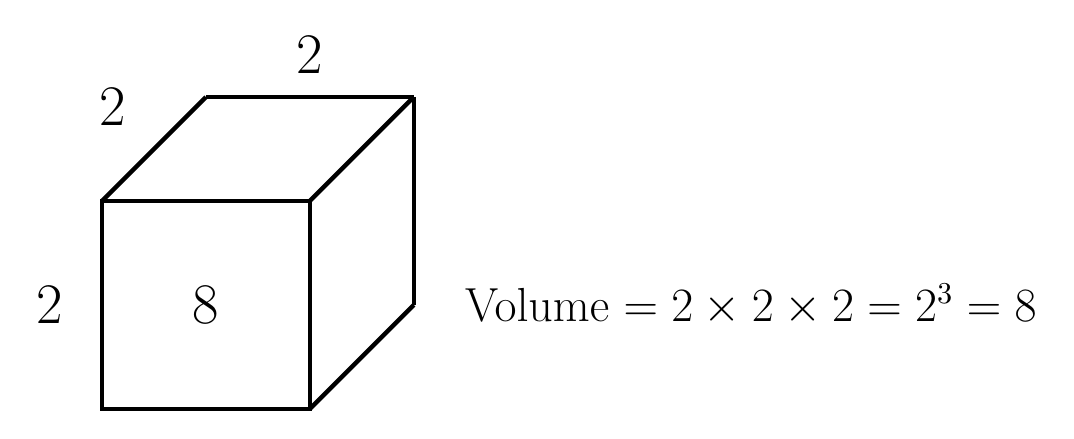
\begin{tikzpicture}[scale=0.66]
% Draw square with thick lines
\draw[ultra thick] (0, 0) rectangle (4, 4);
%\draw[ultra thick, fill=lightgray] (0, 0) rectangle (4, 4);
% Place "8" in the center with larger font size
\node at (2, 2) {\fontsize{20}{24}\selectfont 8};
% Place "2" to the left of the square with larger font size
\node at (-1, 2) {\fontsize{20}{24}\selectfont 2};
% Draw line from top left of square with thick line
\draw[ultra thick] (0, 4) -- (2, 6);
% Place "2" above the line with larger font size
\node at (0.2, 5.8) {\fontsize{20}{24}\selectfont 2};
% Draw line from top right of square with thick line
\draw[ultra thick] (4, 4) -- (6, 6);
% Connect the two lines with a horizontal line with thick line
\draw[ultra thick] (2, 6) -- (6, 6);
% Place "2" above the line with larger font size
\node at (4, 6.8) {\fontsize{20}{24}\selectfont 2};
% Shade the area with gray
%\fill[gray] (0, 4) -- (2, 6) -- (6, 6) -- (4, 4) -- cycle;
% Draw line from bottom right of square with thick line
\draw[ultra thick] (4, 0) -- (6, 2);
% Draw vertical line from the end of the previous line with thick line
\draw[ultra thick] (6, 2) -- (6, 6);
% Shade the area with lighter dark gray
%\fill[darkgray] (4, 0) -- (6, 2) -- (6, 6) -- (4,4) -- cycle;
% Write volume equation to the right with larger font size
\node[right] at (6.8, 2) {\fontsize{16}{19}\selectfont Volume $= 2 \times 2 \times 2 = 2^3 = 8$};
\end{tikzpicture}
\vspace{28pt}

\section*{Roots}

Sometimes you only have a power of a number and you want to find out the root that it started with. Just like you can find the power of a number, you can also find the root.\\

This is called 'taking the root.'\\

If you start with a root of 3 and multiply it by itself 3 times, you get $3 \times 3 \times 3 = 27$, the third power of 3. The number that you have to multiply by itself 3 times to get 27, is 3, so 3 is the third root of 27.\\

Say you are asked to find the fourth root 256. That means you need to find what number, when multiplied by itself 4 times, gives  256.
\begin{align*}
4^1 &= 4\\
4^2 &= 4 \times 4 = 16\\
4^3 &= 4 \times 4 \times 4 = 64\\
4^4 &= 4 \times 4 \times 4 \times 4 = 256
\end{align*}

As you can see, 256 is the fourth power of 4, so 4 is the fourth root of 256.\\

Here is a list of the first powers of 3 :

\begin{center}
$3^1 = 3$
\end{center}
The first power of 3 is just 3, so the first root of 3 is also just 3.

\begin{center}
$3^2 = 3 \times 3 = 9$
\end{center}
3 raised to the second power is 9, so the second root of 9 is 3.

\begin{center}
$3^3 = 3 \times 3 \times 3 = 27$
\end{center}
3 raised to the third power is 27, so third root of 27 is 3.

\begin{center}
$3^4 = 3 \times 3 \times 3 \times 3 = 81$
\end{center}
3 raised to the fourth power is 81, so the fourth root of 81 is 3.

\begin{center}
$3^5 = 3 \times 3 \times 3 \times 3 \times 3 = 243$
\end{center}
3 raised to the fifth power is 243, so the fifth root of 243 is 3.

\item Write out the first 6 powers of 2.
\item What is the 6\textsuperscript{th} root of 64?
\item What is the 4\textsuperscript{th} root of 16?
\item What is the 5\textsuperscript{th} root of 32?

\subsection*{Radicals}

There is a special symbol \raisebox{.8ex}{$\sqrt{}$} used for working with the roots of numbers. The Latin word for root is 'radical' and it is where the radical or root symbol \raisebox{.8ex}{$\sqrt{}$} comes from, being a sort of stretched out letter r.

\item What does radical mean, in your own words?
\item Use radical in a sentence.

\paragraph{Radicand}
The value inside the radical symbol, the number for which the root is being taken, is the radicand.

\item What does radicand mean, in your own words?
\item Use radicand in a sentence.

You write the radical \raisebox{.8ex}{$\sqrt{}$} symbol and the radicand with a line along the top of it. The number to the left of the radical symbol that indicates which root is to be taken is called the index or the order or the degree of the root.\\

\begin{center}
\raisebox{3ex}{index $\longrightarrow$} {\fontsize{40}{44}\selectfont {$\sqrt[5]{243} = 3$}}
\raisebox{1ex}{$\ \longleftarrow$ root}
\end{center}

$\sqrt[5]{243} = 3$ means that 3 is the number which multiplied by itself 5 times is 243. In other words, the 5\textsuperscript{th} root of 243 is 3.

\item what does the \raisebox{.8ex}{$\sqrt{}$} root symbol mean?
\item What does $\sqrt[4]{2401}=7$ mean?
\item Using the root symbol, write that the 4\textsuperscript{th} root of 256 is 4.

\subsection*{Square Roots}

The square of a number is the second power of the number, so the second root of a number is the square root.\\

For a square with an area of 4, the length of it’s sides must be 2. The square root of 4 is 2.

\begin{figure}
  \centering
  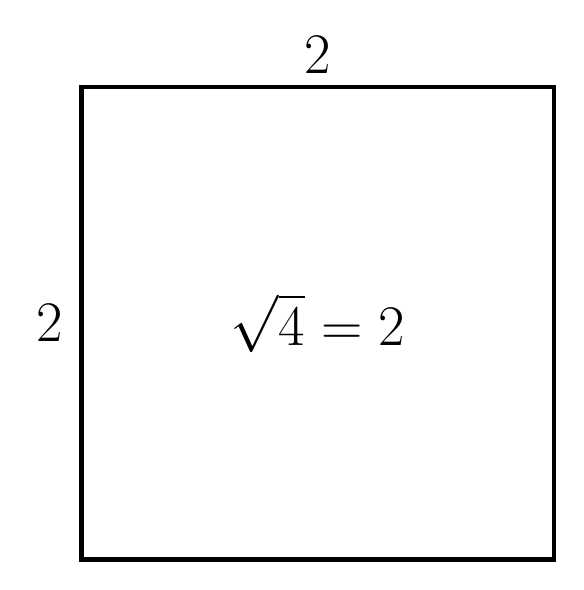
\begin{tikzpicture}
    \draw [ultra thick](0,0) rectangle (6,6);
%    \fill[lightgray] (0,0) rectangle (6,6);
    \node at (3,3) {\fontsize{20}{24}\selectfont $\sqrt{4} = 2$};
    \node at (-0.4,3) {\fontsize{20}{24}\selectfont 2};
    \node at (3,6.4) {\fontsize{20}{24}\selectfont 2};
  \end{tikzpicture}
  \quad
  \begin{minipage}{5cm}
    \[
    \text{Area} = 2 \times 2 = 2^2 = 4
    \]
  \end{minipage}
\end{figure}

If you see the $\sqrt{}$ symbol written without an index then its a square root.  $\sqrt[2]{16} = 4$ is just written as $\sqrt{16} = 4.$ It’s the most commonly used root so the 2 isn’t written unless there is some special reason.

\item In your own words, what is a square root?
\item Why is the second root called the square root?
\item Why isn't the 2 written next to the root symbol of a square root?
\item What does $\sqrt{4}=2$ mean?

\subsection*{Cube Roots}
\begin{align*}
27 &= 3^3\\
9 &= 3^2\\
3 &= 3^1
\end{align*}

The cube of a number is its third power, and its third root is called the cube root.\\

A cube with a volume of 27 must have sides with lengths of 3, so the cube root of 27 is 3.\\

\vspace{28pt}
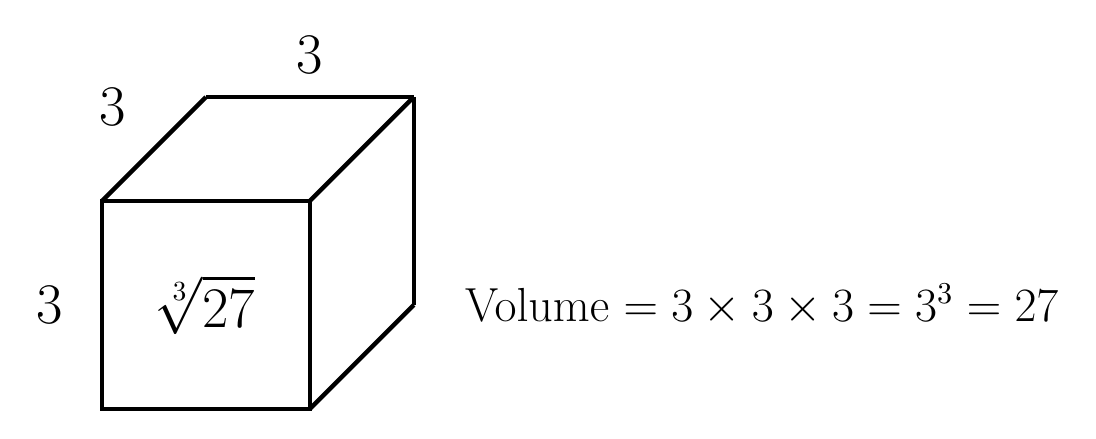
\begin{tikzpicture}[scale=0.66]
% Draw square with thick lines
%\draw[ultra thick, fill=lightgray] (0, 0) rectangle (4, 4);
\draw[ultra thick] (0, 0) rectangle (4, 4);
% Place "8" in the center with larger font size
\node at (2, 2) {\fontsize{20}{24}\selectfont $\sqrt[3]{27}$};
% Place "2" to the left of the square with larger font size
\node at (-1, 2) {\fontsize{20}{24}\selectfont 3};
% Draw line from top left of square with thick line
\draw[ultra thick] (0, 4) -- (2, 6);
% Place "2" above the line with larger font size
\node at (0.2, 5.8) {\fontsize{20}{24}\selectfont 3};
% Draw line from top right of square with thick line
\draw[ultra thick] (4, 4) -- (6, 6);
% Connect the two lines with a horizontal line with thick line
\draw[ultra thick] (2, 6) -- (6, 6);
% Place "2" above the line with larger font size
\node at (4, 6.8) {\fontsize{20}{24}\selectfont 3};
% Shade the area with gray
%\fill[gray] (0, 4) -- (2, 6) -- (6, 6) -- (4, 4) -- cycle;
% Draw line from bottom right of square with thick line
\draw[ultra thick] (4, 0) -- (6, 2);
% Draw vertical line from the end of the previous line with thick line
\draw[ultra thick] (6, 2) -- (6, 6);
% Shade the area with lighter dark gray
%\fill[darkgray] (4, 0) -- (6, 2) -- (6, 6) -- (4,4) -- cycle;
% Write volume equation to the right with larger font size
\node[right] at (6.8, 2) {\fontsize{16}{19}\selectfont Volume $= 3 \times 3 \times 3 = 3^3 = 27$};
\end{tikzpicture}

\vspace{28pt}
You would write $\sqrt[3]{27} = 3$.

\item What is a cube root?
\item Why is the third root called a cube root?
\item Write that the cube root of 27 is 3.

\end{enumerate}

\section*{Practice}

\begin{enumerate}
\item What is 2 to the power of 4?\\
\item What is the square root of 64?\\
\item What is the cube root of 27?\\
\item What is 5 to the power of 3?\\
\item What is the fourth power of 2?\\
\item What is 3 raised to the fourth power?\\
\item What is the fourth root of 81?\\
\item What is 4 cubed?
\end{enumerate}

\subsection*{Answers}

\begin{enumerate}
\item $2^4 = 2 \times 2 \times 2 \times 2 = 16$\\
\item $\sqrt{64} = 8$\\
\item $\sqrt[3]{27} = 3$\\
\item $5^3 = 5 \times 5 \times 5 = 125$\\
\item $2^4 = 2 \times 2 \times 2 \times 2 = 16$\\
\item $3^4 = 3 \times 3 \times 3 \times 3 = 81$\\
\item $3^4 = 81\ \text{so}\ \sqrt[4]{81} = 3$\\
\item $4^3 = 4 \times 4 \times 4 = 64$

\section*{More Practice}

\subsection*{Powers of Numbers}
\begin{enumerate}
\item Define what a power is in mathematics.
\item Explain why we use the notation $3^5$ instead of writing out $3 \times 3 \times 3 \times 3 \times 3$.
\item Calculate the value of $2^3$.
\item Express $5^2$ in words.
\item If $x$ is raised to the power of 4, how would you write it?
\item What is the result of $10^3$?
\item Express the fourth power of 6 in mathematical notation.
\item What is the fifth power of 2.
\item Can you find the eighth power of 10?
\item Read the following powers out loud: $4^3$, $6^2$, $9^4$, $2^5$, $10^8$.
\item Explain the different ways you can verbally express a number with an index (e.g., "3 to the power of 5").
\item Calculate the value of $7^2$ and read it aloud using one of the verbal expressions.
\end{enumerate}

\subsection*{Roots of Numbers}
\begin{enumerate}
\item What is the relationship between the root and the power of a number.
\item Use the word "root" in a sentence related to mathematics.
\item Calculate the roots of the following numbers: $\sqrt{16}$, $\sqrt{25}$, $\sqrt[3]{64}$.
\item Write the fourth root of 81.
\item Find the third root of 125.
\end{enumerate}

\subsection*{Index}
\begin{enumerate}
\item Define what an index is in mathematics.
\item Use the word "index" in a sentence.
\item Explain how the index relates to the power of a number.
\item Calculate the fourth power of 3. What is the index?
\item What is the index in $2^{12}$?
\item Describe what "indices" are in mathematics.
\item Use "indices" in a sentence.
\item Explain why we use "indices" and not "indexes."
\item Find the indices in the expression $2^7 - 3^5$.
\end{enumerate}

\subsection*{Exponent}
\begin{enumerate}
\item What is an "exponent" in mathematics.
\item Use "exponent" in a sentence.
\item What is the origin of the word "exponent."
\item How is an "exponent" related to "power" and "index"?
\item What is the exponent in $10^6$.
\end{enumerate}

\subsection*{The Caret Symbol}
\begin{enumerate}
\item Explain when and why we might use the caret symbol (\textasciicircum) in mathematical expressions.
\item Write five examples of powers of numbers using the caret symbol.
\end{enumerate}

\subsection*{Squares}
\begin{enumerate}
\item Define what a square is.
\item Define "area."
\item Calculate the area of a square with sides of length 6 cm.
\item Explain why multiplying a number by itself is "squaring."
\item Give an example of a real-life situation where understanding squares would be important.
\end{enumerate}

\subsection*{Cubes}
\begin{enumerate}
\item Define what a cube is.
\item Define "volume."
\item Calculate the volume of a cube with side length 4 inches.
\item Explain why raising a number to the third power is called "cubing."
\item Provide an example of a real-life object that can be represented as a cube.
\end{enumerate}

\subsection*{Roots}

\begin{enumerate}
\item How might you go about finding the root of a number?
\item Find the third root of 8.
\item How do roots and powers relate to each other?
\end{enumerate}

\subsection*{Radical}
\begin{enumerate}
\item Define "radical."
\item Explain the origin of the word "radical" and its connection to roots.
\item Using the radical symbol, write the cube root of 64.
\end{enumerate}

\subsection*{Radicand}
\begin{enumerate}
\item What is a "radicand."
\item Write the the cube root of 27 and label the radicand.
\end{enumerate}

\subsection*{Square Roots}
\begin{enumerate}
\item Explain the concept of a square root.
\item Why is the second root called the "square root"?
\item What is the square root of 81.
\end{enumerate}

\subsection*{Cube Roots}
\begin{enumerate}
\item Describe what a cube root is.
\item Why is the third root referred to as the "cube root"?
\item What is the cube root of 64.
\item What could be a real-world example where understanding cube roots is valuable.
\end{enumerate}

\end{document}
